\section{Related Work}

In this section, we discuss studies applicable to virtual reality based text entry.
For a full review of text entry methods, see~\cite{mackenzie2002text, zhai2005search, Buxton2011}.

\subsection{Novel QWERTY Keyboards}
Researchers have leveraged a users' familiarity with the QUERTY~\cite{noyes1983qwerty} keyboard to make their novel devices easier to use.
The Half-QWERTY keyboard~\cite{matias1993half} is arm-mounted and has a reduced size by using only half of a QWERTY keyboard.
The Pinch Gloves~\cite{bowman2002text} controls a virtual keyboard with hand rotations and finger-mounted buttons.
Another glove, KITTY~\cite{Kuester:2005:TKI:1101616.1101635} uses the tapping of contacts on each finger with the thumb to mimic a keyboard.
DigiTap~\cite{Pratorius:2014:DEV:2671015.2671029} is a similar idea but uses a wrist mounted camera instead of a glove.

\subsection{Word Gesture Keyboards}
Word gesture keyboards such as ShapeWriter~\cite{zhai2012word,Zhai:2009:SIL:1520340.1520380} and SHARK 2~\cite{kristensson2004shark}, are gesture based text input methods.
Words are written through a gesture that links the letters of the intended word on a soft keyboard. A language model and word prediction is required to select the most likely word from  candidate words.
For out of vocabulary and hard-to-predict words, a deterministic input method is still needed.
VelociTap~\cite{vertanen2015velocitap} takes the predictive model further by only predicting the whole sentence.

\subsection{Gloves and Chording Keyboards}
Other approaches abandon the QWERTY keyboard entirety.
Chording keyboards~\cite{noyes1983chord}, such as Twiddler~\cite{lyons2004twiddler} use a combination of a few keys to produce characters.
Chording is done is done with gloves, such as Chording Glove~\cite{rosenberg1999chording}.
The VirtualPhonepad~\cite{ahn2006virtualphonepad} imitates text entry via a $3\times3$ mobile phone keypad.
Virtual Notepad~\cite{poupyrev1998virtual} allows for creating handwritten annotations in virtual reality.
Connecting the Dots~\cite{frees2006connecting} approximates handwriting by having users connect dots on a $3\times3$ virtual dot matrix to scribe a single character.

In a literature review, the Pinch Gloves, pen and tablet, chording keyboard, and a speech-based are compared~\cite{bowman2002text}.
The pen and tablet and speech are fastest.  The pen and tablet had the fewest errors.
The comparison was done before specialized virtual reality input device were invented.

\subsection{Home Entertainment Input Devices}
Text entry methods is sought after in other application areas, such as home entertainment systems.
SpeeG~\cite{hoste2012speeg} is a Kinect~\cite{geerse2015kinematic} version of Speech Dasher~\cite{vertanen2010speech} text input technique.
The user speaks and then corrects mistakes using an interface that scrolls through the recognized text as well as alternatives.
SpeeG2~\cite{hoste2013speeg2} uses a grid instead of a scroll.

\subsection{Speech recognition}
Spoken language is effective for human-human interaction but often has severe limitations when applied to human-computer interaction.
Speech is slow for presenting information and interferes significantly with other cognitive tasks~\cite{shneiderman2000limits}.

Speech recognition is limited when typing passwords, names, and URLs~\cite{TODO}. 
The lack of user acceptance is also due to issues such as privacy, the perception of bothering others, the awkwardness of speaking to a machine~\cite{sawhney2000nomadic}.
Some users find voice as unreliable especially when the accent or ambient sound negatively affect accuracy.
Studies have shown that users find it ``harder to talk and think than type and think" and considered the keyboard to be more ``natural" than speech for text entry ~\cite{Karat:1999:PEC:302979.303160}.

In virtual reality, a Japanese speech-based entry system represents candidate words recognized by the speech recognition engine as blocks that can be moved around in the virtual enviroment~\cite{osawa2002multimodal}. 

For mobile phones, speech entry is three times faster than typing for English and Mandarin~\cite{ruan2016speech}.  
In this experimental setup, participants were given a set of phrases to type and speak.
The phrases are given ahead of time, but normal speech is filled with hesitations, repetitions, changes of subject in the middle of an utterance~\cite{forsberg2003speech} as the user thinks.
This could lead to an unrealistic accuracy for speech.  
The study also excludes punctuation marks and capital letters from the phrases.
Generating accurate punctuation  automatically with speech input is not yet possible and must be done manually~\cite{chen1999speech}.

\subsection{Gaze Directed Typing}
Gaze directed typing is the main text input method used today in systems such as Oculus G earVR. A main advantage of this method is that it uses the available hardware and does not require an additional device. This method is slow~\cite{card1983psychology, mackenzie1992fitts} and inconvenient since the whole head has to be moved for each character.
Moving the head while the VR scene remains static also often causes nausea or dizziness~\cite{atienza2016interaction}.   

\subsection{Text Input with Virtual Reality Controllers}
While early, input methods and controllers are being developed specifically for use in virtual reality.
FaceTouch~\cite{Gugenheimer:2016:FTI:2851581.2890242} has the backside of the head mounted display that as a touch sensitive surface.
The user selects virtual content by touching the corresponding location on backside of the display.
It is useful but only for short periods of time before the users' arms get tired.

Belt~\cite{dobbelstein2015belt} is a novel unobtrusive input device for wearable displays that has a touch surface encircling a users' hip.
The wide input space for a horizontal spatial mapping but suffers from low throughput, arm fatigue, and social acceptance.
Nenya~\cite{ashbrook2011nenya} uses a finger ring as an input mechanism that is always available.
It is fast to access, allows analog input, and is socially acceptable by being embodied in a commonly worn item.

Industry has started to standardize around a virtual reality controller.  HTC, Facebook, and Google have all released a virtual reality hardware design.
Each includes a controller, shown in Figure~~\ref{fig:controllers}.
They all similar in the they all contain a rotational tracking, a way to track the thumb through either joystick or touchpad, and at least four buttons.
Vive and Oculus use an absolute tracking system to minimizing sensor drift and to allow for rotational and translational tracking~\cite{hilfert2016low}.
The Daydream controller, shown in Figure~\ref{fig:controllerDaydream}, in only for a single hand whereas the others have a controller for each hand.
SwipeVR is implemented using the Vive but could be implemented on the other two.

\newcommand{\ra}[1]{\renewcommand{\arraystretch}{#1}}


\begin{table*}\centering
\ra{1.3}
\begin{tabular}{@{}rrrrrr@{}}\toprule
						& $Speech$ 		& $Gaze$ 		& $Mobile$		& $SwipeVR$  \\
\midrule
$Positioning$			&				& absolute		& absolute		& relative	  		\\
$Hardware$ 				&microphone 	& HMD \& button	& touch screen	& controller		\\
$Keys$ 					&				& 26+			& 26+			& 6					\\
$Special~Characters$ 	&				& \checkmark	& \checkmark	& \checkmark		\\
$Granulatiry$ 			&word			& character		& character		& word or character	\\
$Hands$ 				& 0				& 1				& 1 or 2		& 1					\\
$Real-Time~Feedback$ 	& word			& character		& character		& word				\\
$Cursor~Mode$ 			& NA			& persistent	& NA			& snap-to-home		\\
$Silent$ 				&				& \checkmark	& \checkmark	&\checkmark			\\
$Muscle$ 				& vocal chords	& neck			& fingers		& thumb			\\
$WPM$					& \%\cite{sppechTBA} & \%		& \%			& \%\\
$Error~Rate$			& \%\cite{sppechTBA} & \%		& \%			& \%\\

%    Correction Method		& X 			& X 			& X				& 	\checkmark		\\ 

\bottomrule
\end{tabular}
\caption{Ontology of input methods.}
\label{table:ontology}
\end{table*}

\begin{figure}
  \centering
	\begin{subfigure}{.4\columnwidth}
  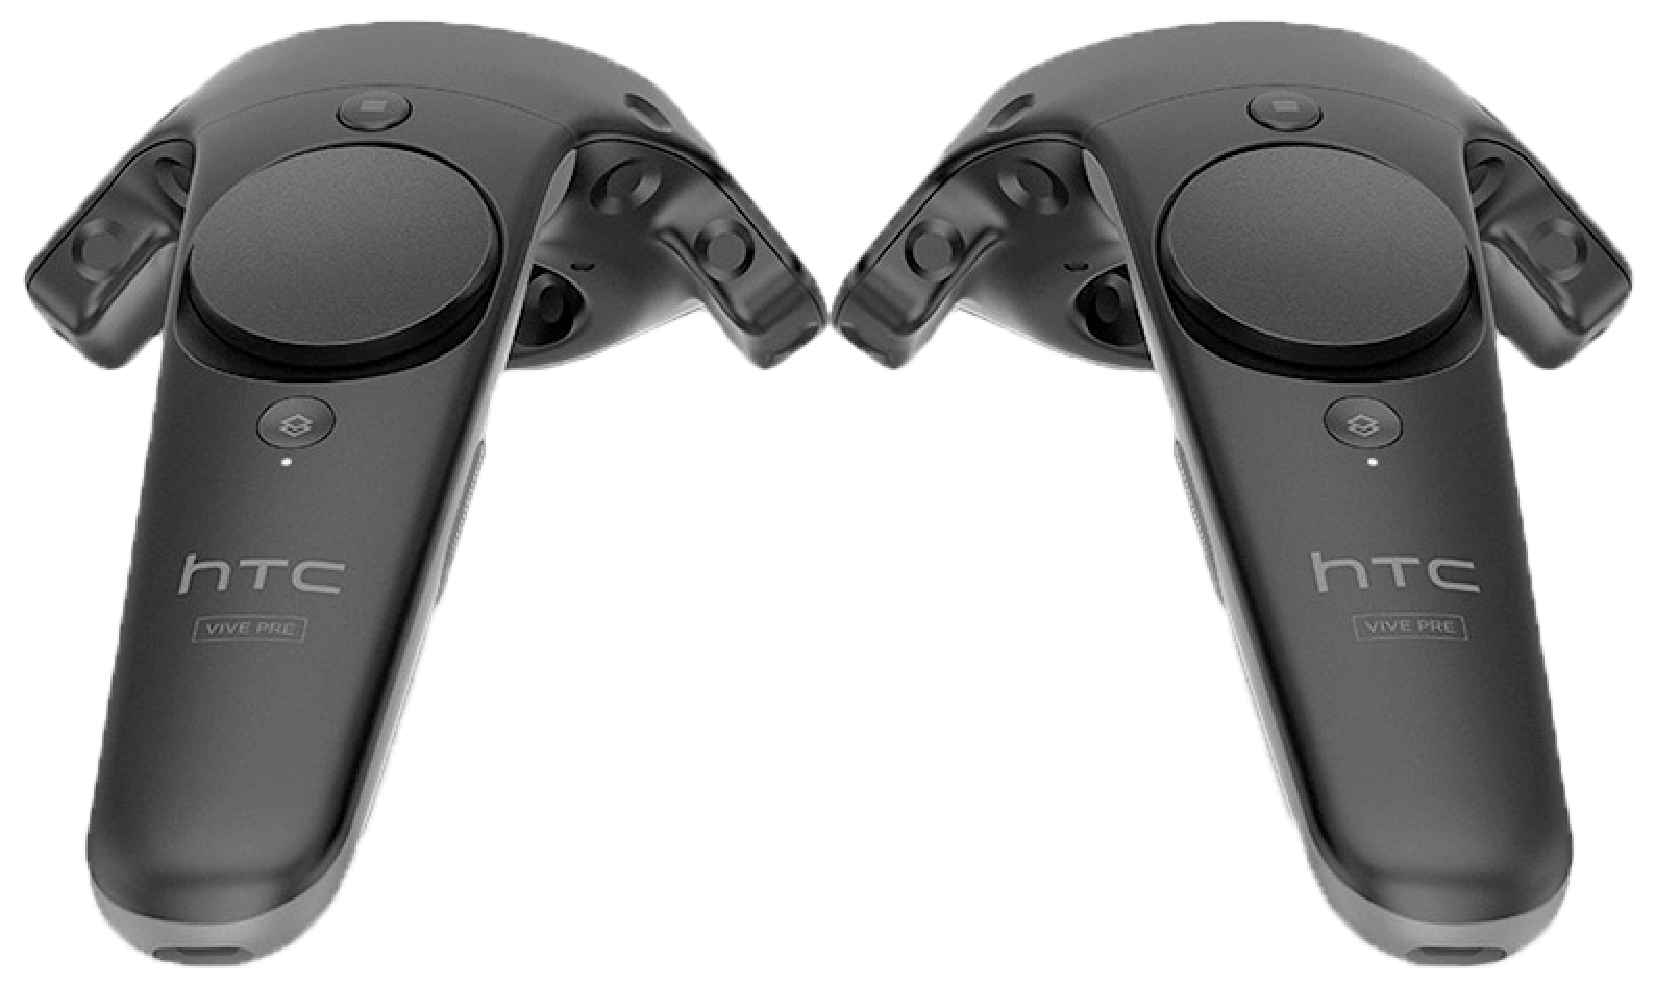
\includegraphics[width=\textwidth]{figures/controllerVive}
  \caption{HTC's Vive }\label{fig:controllerVive}
  \end{subfigure}
  \\
  \begin{subfigure}{.4\columnwidth}
  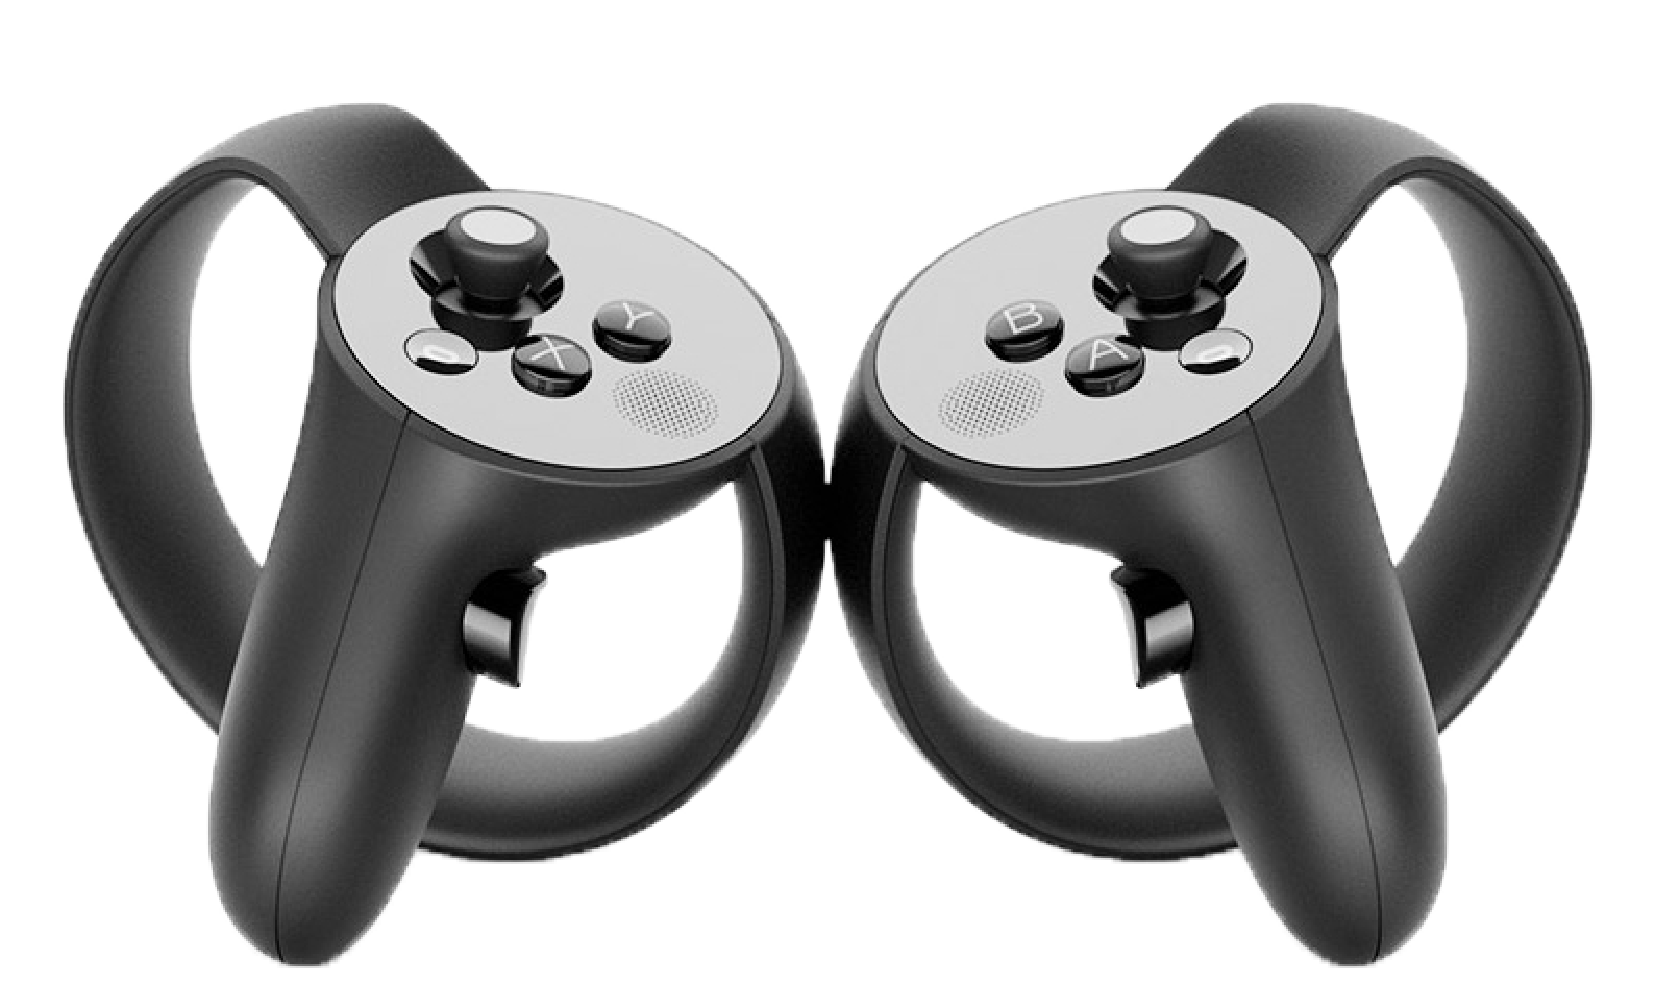
\includegraphics[width=\textwidth]{figures/controllerOculus}
  \caption{Facebook's Oculus}\label{fig:controllerOculus}
  \end{subfigure}
  \\
  \begin{subfigure}{.4\columnwidth}
  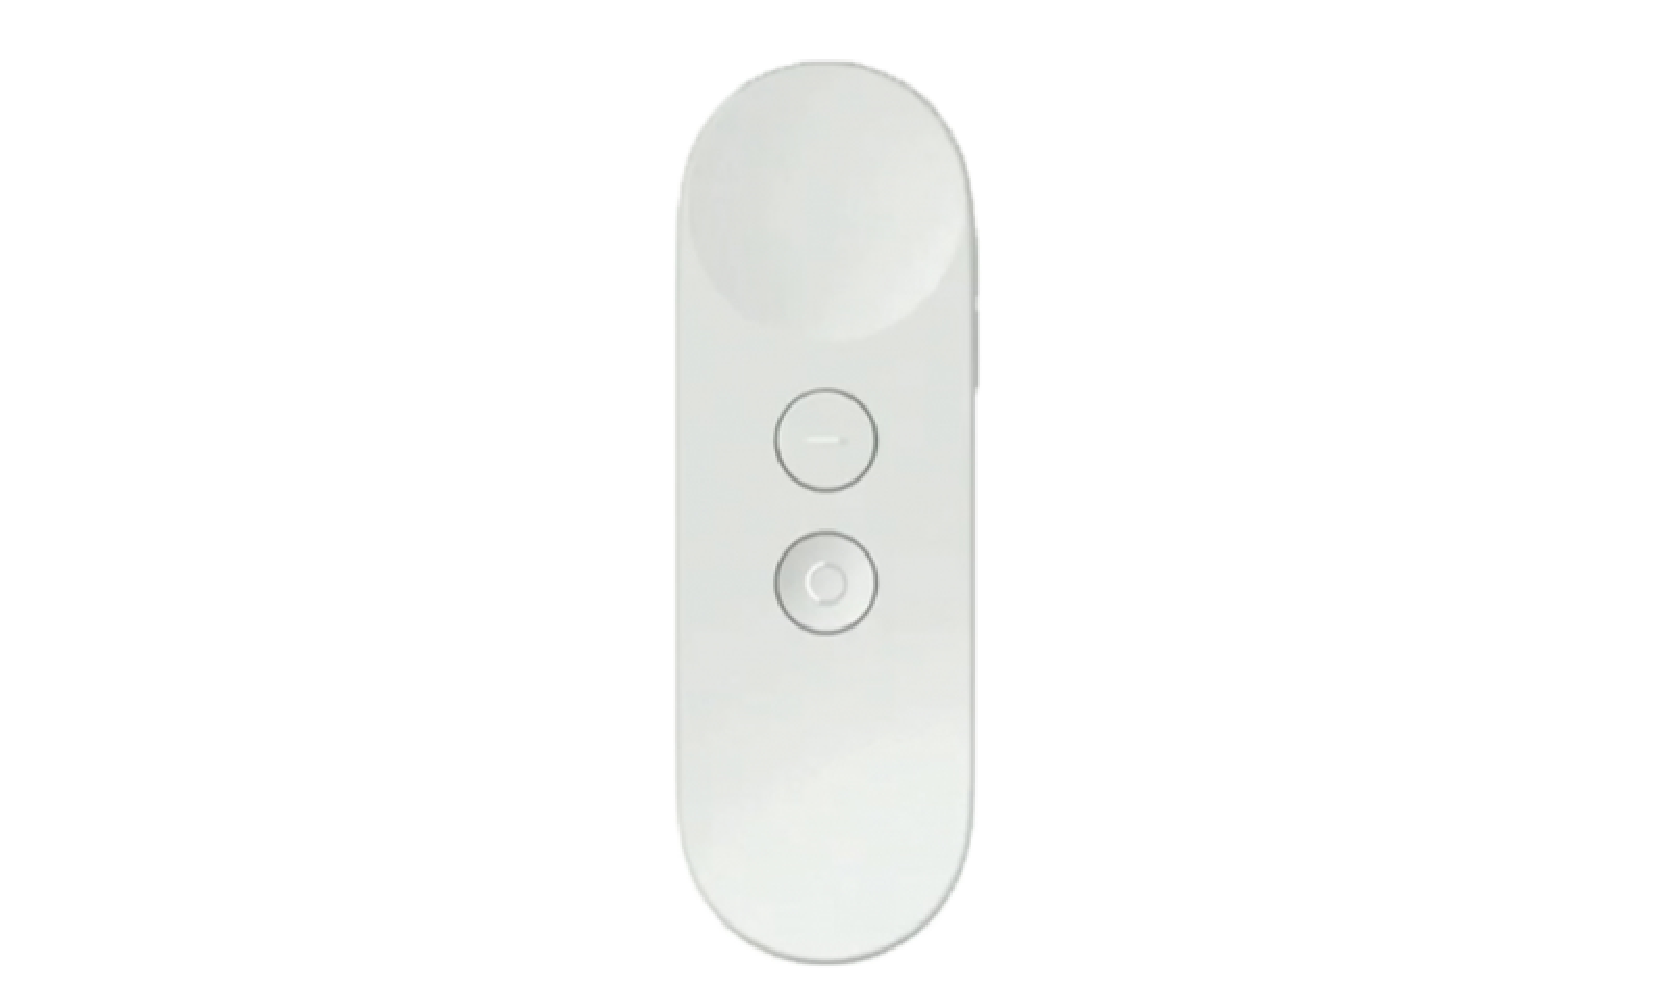
\includegraphics[width=\textwidth]{figures/controllerDaydream}
  \caption{Google's Daydream}\label{fig:controllerDaydream}
  \end{subfigure}
  \caption{
  Industry is standardizing on some of the important components for virtual reality controllers.
  The three major controllers shown above all contain a way to track the thumb, at least 3 degrees of freedom tracking  (rotational), and at least four buttons.
  The Vive (\subref{fig:controllerVive}) and the Oculus (\subref{fig:controllerOculus}) use room-scale tracking to give 6 degrees of freedom (rotation and translation).  
  Many virtual reality systems today are released with a controller for each hand.  
  The Vive and Daydream (\subref{fig:controllerDaydream}) employ a thumb track pad to capture finger movement.
  Oculus controller uses joysticks instead.
  The system described in this paper is implemented using the Vive and could be implemented on the other two.
  }~\label{fig:controllers}

\end{figure}



